% Options for packages loaded elsewhere
\PassOptionsToPackage{unicode}{hyperref}
\PassOptionsToPackage{hyphens}{url}
%
\documentclass[
]{book}
\usepackage{lmodern}
\usepackage{amssymb,amsmath}
\usepackage{ifxetex,ifluatex}
\ifnum 0\ifxetex 1\fi\ifluatex 1\fi=0 % if pdftex
  \usepackage[T1]{fontenc}
  \usepackage[utf8]{inputenc}
  \usepackage{textcomp} % provide euro and other symbols
\else % if luatex or xetex
  \usepackage{unicode-math}
  \defaultfontfeatures{Scale=MatchLowercase}
  \defaultfontfeatures[\rmfamily]{Ligatures=TeX,Scale=1}
\fi
% Use upquote if available, for straight quotes in verbatim environments
\IfFileExists{upquote.sty}{\usepackage{upquote}}{}
\IfFileExists{microtype.sty}{% use microtype if available
  \usepackage[]{microtype}
  \UseMicrotypeSet[protrusion]{basicmath} % disable protrusion for tt fonts
}{}
\makeatletter
\@ifundefined{KOMAClassName}{% if non-KOMA class
  \IfFileExists{parskip.sty}{%
    \usepackage{parskip}
  }{% else
    \setlength{\parindent}{0pt}
    \setlength{\parskip}{6pt plus 2pt minus 1pt}}
}{% if KOMA class
  \KOMAoptions{parskip=half}}
\makeatother
\usepackage{xcolor}
\IfFileExists{xurl.sty}{\usepackage{xurl}}{} % add URL line breaks if available
\IfFileExists{bookmark.sty}{\usepackage{bookmark}}{\usepackage{hyperref}}
\hypersetup{
  pdftitle={Time Series for Beginners},
  pdfauthor={Jake Esprabens, Ari Arango, Joshua Kim},
  hidelinks,
  pdfcreator={LaTeX via pandoc}}
\urlstyle{same} % disable monospaced font for URLs
\usepackage{color}
\usepackage{fancyvrb}
\newcommand{\VerbBar}{|}
\newcommand{\VERB}{\Verb[commandchars=\\\{\}]}
\DefineVerbatimEnvironment{Highlighting}{Verbatim}{commandchars=\\\{\}}
% Add ',fontsize=\small' for more characters per line
\usepackage{framed}
\definecolor{shadecolor}{RGB}{248,248,248}
\newenvironment{Shaded}{\begin{snugshade}}{\end{snugshade}}
\newcommand{\AlertTok}[1]{\textcolor[rgb]{0.94,0.16,0.16}{#1}}
\newcommand{\AnnotationTok}[1]{\textcolor[rgb]{0.56,0.35,0.01}{\textbf{\textit{#1}}}}
\newcommand{\AttributeTok}[1]{\textcolor[rgb]{0.77,0.63,0.00}{#1}}
\newcommand{\BaseNTok}[1]{\textcolor[rgb]{0.00,0.00,0.81}{#1}}
\newcommand{\BuiltInTok}[1]{#1}
\newcommand{\CharTok}[1]{\textcolor[rgb]{0.31,0.60,0.02}{#1}}
\newcommand{\CommentTok}[1]{\textcolor[rgb]{0.56,0.35,0.01}{\textit{#1}}}
\newcommand{\CommentVarTok}[1]{\textcolor[rgb]{0.56,0.35,0.01}{\textbf{\textit{#1}}}}
\newcommand{\ConstantTok}[1]{\textcolor[rgb]{0.00,0.00,0.00}{#1}}
\newcommand{\ControlFlowTok}[1]{\textcolor[rgb]{0.13,0.29,0.53}{\textbf{#1}}}
\newcommand{\DataTypeTok}[1]{\textcolor[rgb]{0.13,0.29,0.53}{#1}}
\newcommand{\DecValTok}[1]{\textcolor[rgb]{0.00,0.00,0.81}{#1}}
\newcommand{\DocumentationTok}[1]{\textcolor[rgb]{0.56,0.35,0.01}{\textbf{\textit{#1}}}}
\newcommand{\ErrorTok}[1]{\textcolor[rgb]{0.64,0.00,0.00}{\textbf{#1}}}
\newcommand{\ExtensionTok}[1]{#1}
\newcommand{\FloatTok}[1]{\textcolor[rgb]{0.00,0.00,0.81}{#1}}
\newcommand{\FunctionTok}[1]{\textcolor[rgb]{0.00,0.00,0.00}{#1}}
\newcommand{\ImportTok}[1]{#1}
\newcommand{\InformationTok}[1]{\textcolor[rgb]{0.56,0.35,0.01}{\textbf{\textit{#1}}}}
\newcommand{\KeywordTok}[1]{\textcolor[rgb]{0.13,0.29,0.53}{\textbf{#1}}}
\newcommand{\NormalTok}[1]{#1}
\newcommand{\OperatorTok}[1]{\textcolor[rgb]{0.81,0.36,0.00}{\textbf{#1}}}
\newcommand{\OtherTok}[1]{\textcolor[rgb]{0.56,0.35,0.01}{#1}}
\newcommand{\PreprocessorTok}[1]{\textcolor[rgb]{0.56,0.35,0.01}{\textit{#1}}}
\newcommand{\RegionMarkerTok}[1]{#1}
\newcommand{\SpecialCharTok}[1]{\textcolor[rgb]{0.00,0.00,0.00}{#1}}
\newcommand{\SpecialStringTok}[1]{\textcolor[rgb]{0.31,0.60,0.02}{#1}}
\newcommand{\StringTok}[1]{\textcolor[rgb]{0.31,0.60,0.02}{#1}}
\newcommand{\VariableTok}[1]{\textcolor[rgb]{0.00,0.00,0.00}{#1}}
\newcommand{\VerbatimStringTok}[1]{\textcolor[rgb]{0.31,0.60,0.02}{#1}}
\newcommand{\WarningTok}[1]{\textcolor[rgb]{0.56,0.35,0.01}{\textbf{\textit{#1}}}}
\usepackage{longtable,booktabs}
% Correct order of tables after \paragraph or \subparagraph
\usepackage{etoolbox}
\makeatletter
\patchcmd\longtable{\par}{\if@noskipsec\mbox{}\fi\par}{}{}
\makeatother
% Allow footnotes in longtable head/foot
\IfFileExists{footnotehyper.sty}{\usepackage{footnotehyper}}{\usepackage{footnote}}
\makesavenoteenv{longtable}
\usepackage{graphicx,grffile}
\makeatletter
\def\maxwidth{\ifdim\Gin@nat@width>\linewidth\linewidth\else\Gin@nat@width\fi}
\def\maxheight{\ifdim\Gin@nat@height>\textheight\textheight\else\Gin@nat@height\fi}
\makeatother
% Scale images if necessary, so that they will not overflow the page
% margins by default, and it is still possible to overwrite the defaults
% using explicit options in \includegraphics[width, height, ...]{}
\setkeys{Gin}{width=\maxwidth,height=\maxheight,keepaspectratio}
% Set default figure placement to htbp
\makeatletter
\def\fps@figure{htbp}
\makeatother
\setlength{\emergencystretch}{3em} % prevent overfull lines
\providecommand{\tightlist}{%
  \setlength{\itemsep}{0pt}\setlength{\parskip}{0pt}}
\setcounter{secnumdepth}{5}
\usepackage{booktabs}
\usepackage[]{natbib}
\bibliographystyle{apalike}

\title{Time Series for Beginners}
\author{Jake Esprabens, Ari Arango, Joshua Kim}
\date{2020-06-12}

\begin{document}
\maketitle

{
\setcounter{tocdepth}{1}
\tableofcontents
}
\hypertarget{preface}{%
\chapter*{Preface}\label{preface}}
\addcontentsline{toc}{chapter}{Preface}

This book is created with an objective to clearly explain the basics of time series analysis. The inspiration came from taking a time series course and constantly getting confused by the theory. Often, time series can be a tricky subject; therefore, this book will try to explain the essentials of time series using R.

Time series is an immense subject with so much to it; therefore, we won't be able to cover all of it in this book. We will solely focus on what we believe is the most important to provide you with the ability to forecast with time series.

Make sure to check out our correspoding API package and Stock Shiny App to explore real world uses of time series. This package will allow you to directly grab the most recent data on stock prices around the world. Moreover, the Shiny App will allow you to visualize and interact with this data as a time series and predict how the stock prices will move in the future!

I recommend installing these 3 packages before we get started:

\begin{Shaded}
\begin{Highlighting}[]
\KeywordTok{library}\NormalTok{(tidyverse)}
\KeywordTok{library}\NormalTok{(ggfortify)}
\KeywordTok{library}\NormalTok{(forecast)}
\end{Highlighting}
\end{Shaded}

\hypertarget{introduction-to-time-series}{%
\chapter{Introduction to Time Series}\label{introduction-to-time-series}}

\hypertarget{what-is-a-time-series}{%
\section{What is a Time Series?}\label{what-is-a-time-series}}

A time series is a series of data points over time. Sounds pretty simple, right?

Let's take a look at an example of time series using real world data. This data set looks at the average global temperature anomalies in celsius per month from January 1950 to December 2016.

Let's see what what this data looks like.

\begin{verbatim}
##    Mean
## 1 -0.30
## 2 -0.26
## 3 -0.06
## 4 -0.21
## 5 -0.12
\end{verbatim}

\textbf{\emph{We must convert the data into a time series object.}} Now we know that this data is monthly and that it started in January 1950 and ended in December 2016. So we must convert it to a time series object, using the \emph{ts()} function in R. It takes in these arguments.

\begin{itemize}
\tightlist
\item
  start = the starting time of the time series
\item
  end = the ending time of the time series
\item
  frequency = the number of observations per unit of time.

  \begin{itemize}
  \tightlist
  \item
    For monthly data, frequency will be 12
  \item
    For quarterly data, frequency will be 4
  \item
    For biannual data, frequency will be 2
  \end{itemize}
\end{itemize}

\begin{Shaded}
\begin{Highlighting}[]
\NormalTok{temp.ts <-}\StringTok{ }\KeywordTok{ts}\NormalTok{(temp, }\DataTypeTok{start =} \DecValTok{1950}\NormalTok{, }\DataTypeTok{end =} \DecValTok{2016}\NormalTok{, }\DataTypeTok{frequency =} \DecValTok{12}\NormalTok{)}
\end{Highlighting}
\end{Shaded}

\begin{verbatim}
##        Jan   Feb   Mar   Apr   May   Jun   Jul   Aug   Sep   Oct   Nov   Dec
## 1950 -0.30 -0.26 -0.06 -0.21 -0.12 -0.06 -0.09 -0.18 -0.10 -0.20 -0.35 -0.20
## 1951 -0.35 -0.44 -0.19 -0.10 -0.02 -0.05  0.00  0.05  0.07  0.06  0.00  0.15
## 1952  0.16  0.12 -0.10  0.02 -0.05 -0.04  0.05  0.07  0.08 -0.04 -0.17 -0.02
\end{verbatim}

As we can see, the data is now a time series object with 804 observations where each observation represents a month from 1950 to 2016.

How would this object look plotted?

There are several ways to plot time series in R, including the base R function \emph{plot()}; however, we will be using the \emph{autoplot()} function from the \textbf{forecast} package.

\begin{Shaded}
\begin{Highlighting}[]
\KeywordTok{autoplot}\NormalTok{(temp.ts, }\DataTypeTok{colour =} \StringTok{"dodgerblue4"}\NormalTok{) }\OperatorTok{+}
\StringTok{  }\KeywordTok{ggtitle}\NormalTok{(}\StringTok{"Average Global Temperature Anomalies Per Month 1950-2016"}\NormalTok{) }\OperatorTok{+}\StringTok{ }
\StringTok{  }\KeywordTok{ylab}\NormalTok{(}\StringTok{"Average Temperature Difference (Celsius)"}\NormalTok{) }\OperatorTok{+}\StringTok{ }
\StringTok{  }\KeywordTok{theme_classic}\NormalTok{()}
\end{Highlighting}
\end{Shaded}

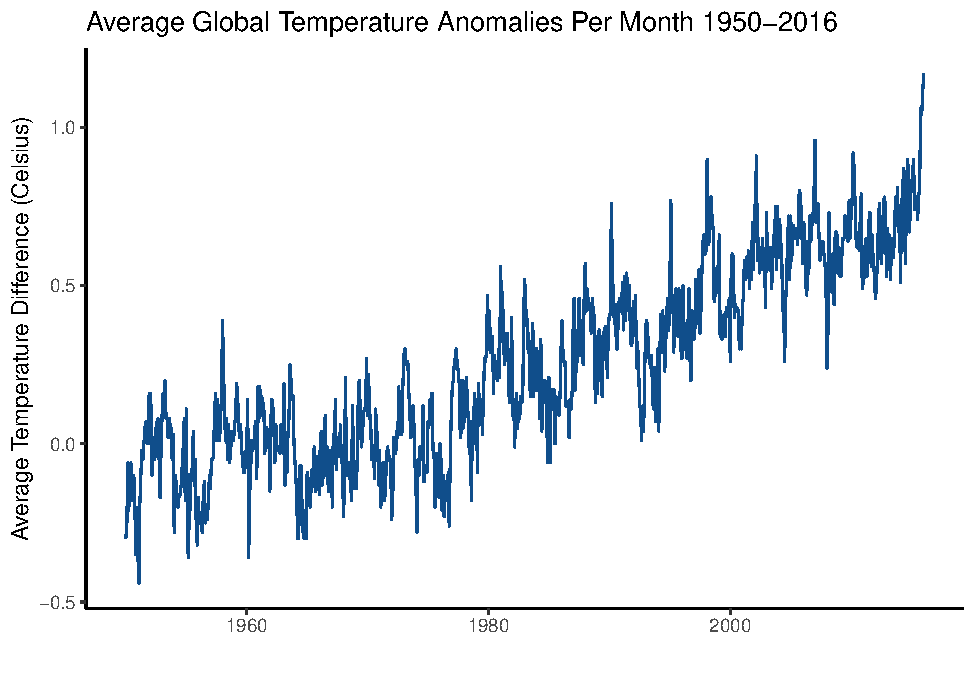
\includegraphics{431-Time-Series_files/figure-latex/unnamed-chunk-6-1.pdf}

What can we take away from this plot?

Well, the first thing you might notice is that the average global temperatue has risen rapidly since about 1970! It also gradually increased from 1950 to 1970. It also staggers a lot all the way through. One might conclude that temperature has increased in the past 66 years! How can you define the changed happening in this time series though? What does the rapid staggering mean? What do you call the upward movement?

\hypertarget{components-of-time-series}{%
\section{Components of Time Series}\label{components-of-time-series}}

What makes up a time series?

Without going into too much notation, a simple additive decomposed model will look like this:

\[x_{t} = m_{t} + s_{t} + e_{t}\]

where:

\begin{itemize}
\tightlist
\item
  \(m_t\) is the trend
\item
  \(s_t\) is the seasonality
\item
  \(e_t\) is the error or random white noise
\end{itemize}

To put it simply, the components of a time series model are defined as:

\begin{itemize}
\tightlist
\item
  trend - the increasing or decreasing values in a series
\item
  seasonality - the repeating short-term cycles in the series
\item
  random white noise - random variation in the series
\end{itemize}

To visualize these in R, you can easily use the base R function, \emph{decompose()}, to produce plots for all three of these components. However, I chose to create my own plots using \textbf{ggplot2}.

\textbf{Trend}

What does the trend plot look like for this global temperature time series?

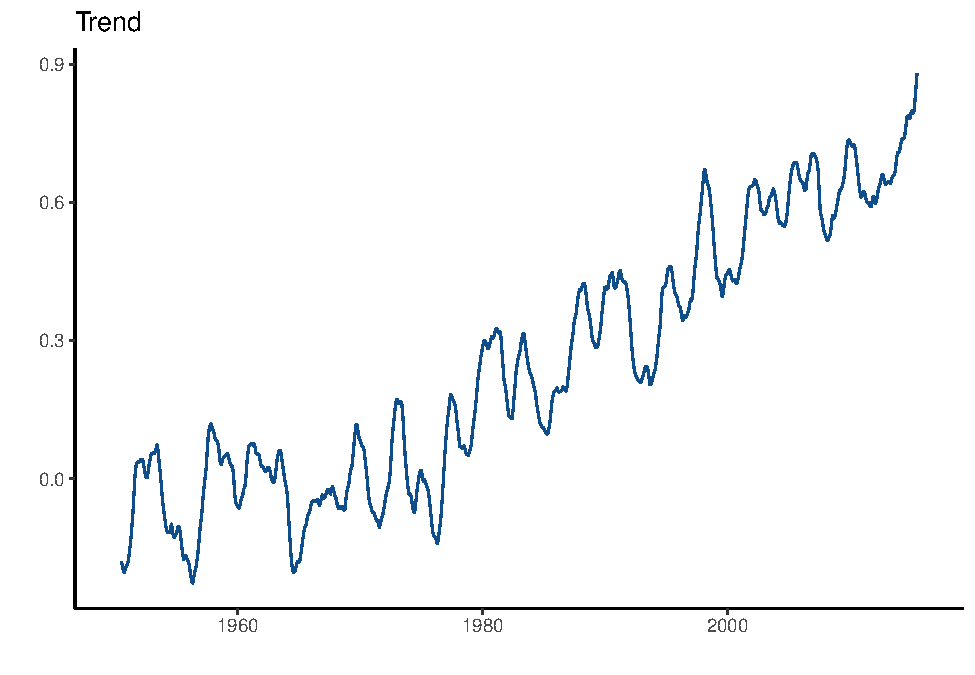
\includegraphics{431-Time-Series_files/figure-latex/unnamed-chunk-8-1.pdf}

As we can see, there is strong upward trend. This means that the temperature is gradually going up since 1950! What if the trend line was going down? Then you would conclude that the temperature is decreasing. What if it stayed constant? Then, you can conclude that there is no trend!

\textbf{Seasonality}

What does the seasonality plot look like for this global temperature time series?

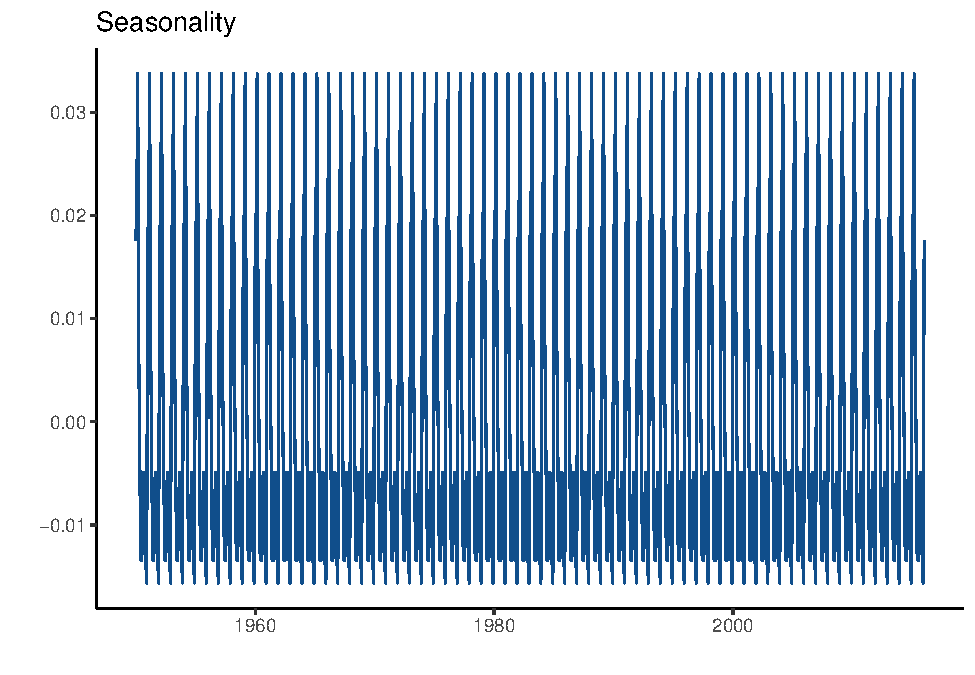
\includegraphics{431-Time-Series_files/figure-latex/unnamed-chunk-9-1.pdf}

In a seasonality plot, you are looking for a common short-term pattern. Seasonality can be caused by many thing depending in the dataset. It is hard to tell if there is seasonality in this time series because of the rapid staggering. Usually, seasonality will be more obvious. An example of seasonality is airline flyers. Many people are often flying in the summer and in the winter for vacation. Thus, that specific time series will see high spikes every 6 months.

\textbf{Random White Noise}

What does the random white noise plot look like for this global temperature time series?

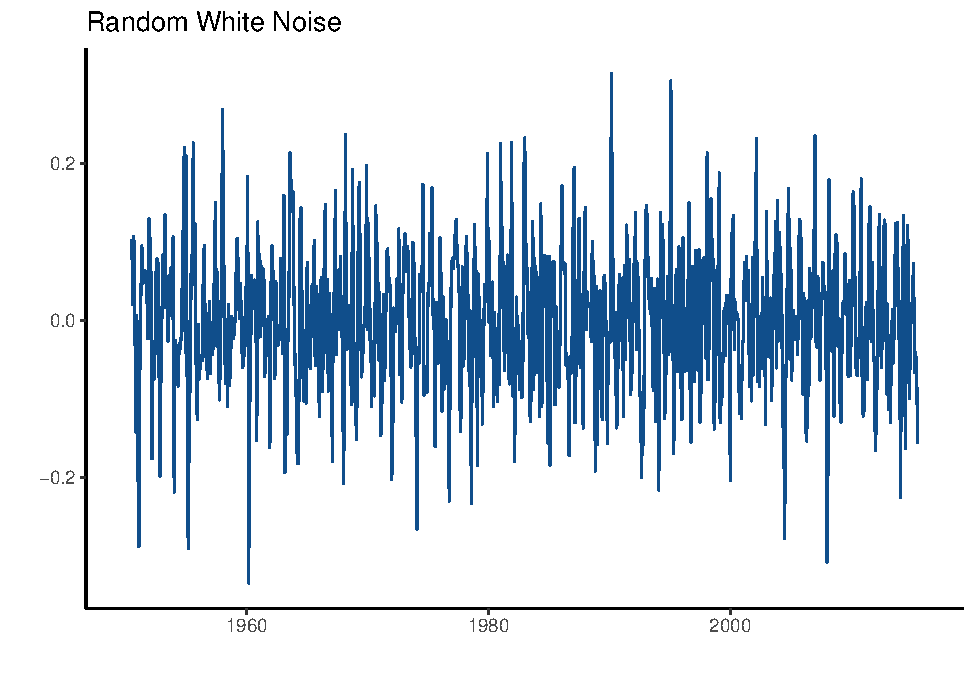
\includegraphics{431-Time-Series_files/figure-latex/unnamed-chunk-10-1.pdf}

Looks pretty random right? That's because it is! This plot illustrates the variation in the time series. This is the unexplained variation that solely happens by chance. This term is similar to the error term in a regression model.

\hypertarget{stationarity}{%
\section{Stationarity}\label{stationarity}}

Stationarity is one of the most important characteristics of a time series. What does it mean for a time series to be stationarity? It is defined by having a constant mean and variance across the time series. A time series needs to be stationary in order for it to make good prediction. We can check if a time series is stationary by looking at the \textbf{autocorrelation function (ACF)}. What exactly is autocorrelation? Autocorrelation basically measures the similarity between observations as a function of the time lag between them.

Let's take a look at the ACF plot of the global temperature time series, using the \emph{acf()} function in R.

\begin{Shaded}
\begin{Highlighting}[]
\NormalTok{acf.plot <-}\StringTok{ }\KeywordTok{acf}\NormalTok{(temp.ts, }\DataTypeTok{lag.max =} \DecValTok{300}\NormalTok{)}
\end{Highlighting}
\end{Shaded}

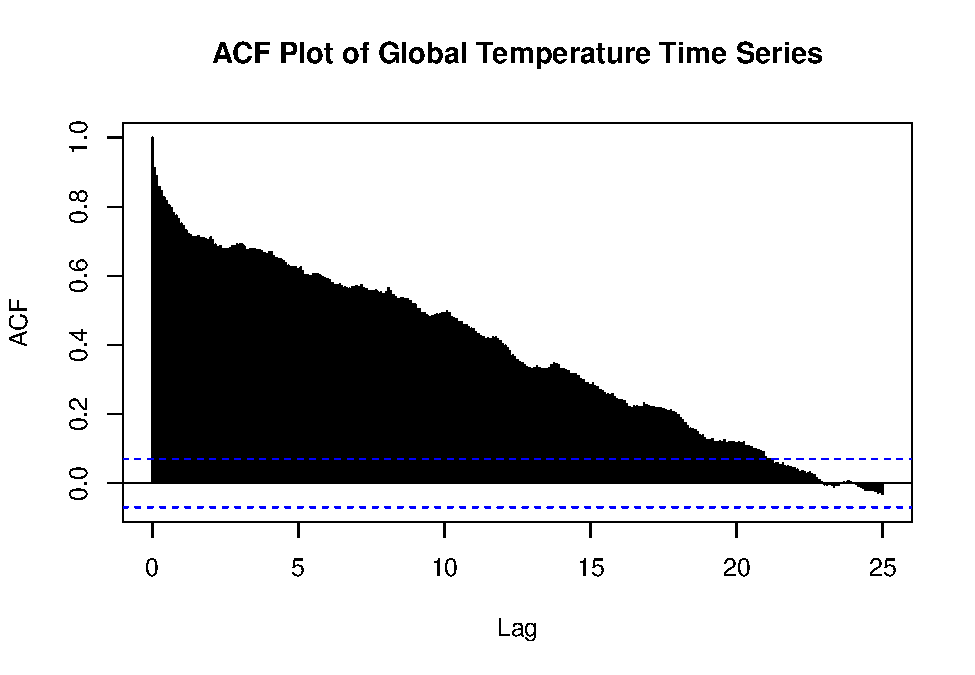
\includegraphics{431-Time-Series_files/figure-latex/unnamed-chunk-12-1.pdf}

What does this mean?

If the series was stationary, we would see basically every line within the blue confidence intervals. However, we see that every spike is out of these lines. This slow decay represents means that there is a trend in the time series, but there is no seasonality!

Here are some common ACF plots you may see:

\begin{itemize}
\tightlist
\item
  Trend and seasonality - Takes a long time decay and also looks similar to a sin graph.
\item
  Trend, but no seasonality - Decays very slowly and the spikes are out of the blue confdience intervals.
\item
  Seasonality, but no trend - Decays quickly and looks similar to a sin graph
\item
  Stationarity - All lines within the blue confidence intervals, besides the first spike.
\end{itemize}

If a time series has trend or seasonality, then it is not stationary. This means that it won't be good for forecasting. What can we do to fix this? We can create new models to represent the time series and make it stationary. We will go over this in the next chapter.

\hypertarget{modelling-time-series}{%
\chapter{Modelling Time Series}\label{modelling-time-series}}

As mentioned before, a time series must be stationary for it to be used to predict well founded values. We will go over several models that we can create in order to allow forecasting.

Please note that the first 3 models we cover, AR, MA, and ARMA, can be used on already stationary time series in order to allow them to predict better values. The remaining models are used on non-stationary time series.

\hypertarget{ar-and-ma}{%
\section{AR and MA}\label{ar-and-ma}}

Two of the most common models in time series are the Autoregressive (AR) models and the Moving Average (MA) models.

\textbf{Autoregressive Model: AR(p)}

The autoregressive model uses observations from preivous time steps as input to a regression equations to predict the value at the next step. The AR model takes in one argument, p, which determines how many previous time steps will be inputted.

The order, p, of the autoregressive model can be deterimined by looking at the \textbf{partial autocorrelation function (PACF)}. The PACF gives the partial correlation of a stationary time series with its own lagged values, regressed of the time series at all shorter lags.

Let's take a look at the PACF plot for the global temperature time series using the \emph{pacf()} function in R.

\begin{Shaded}
\begin{Highlighting}[]
\NormalTok{pacf.plot <-}\StringTok{ }\KeywordTok{pacf}\NormalTok{(temp.ts)}
\end{Highlighting}
\end{Shaded}

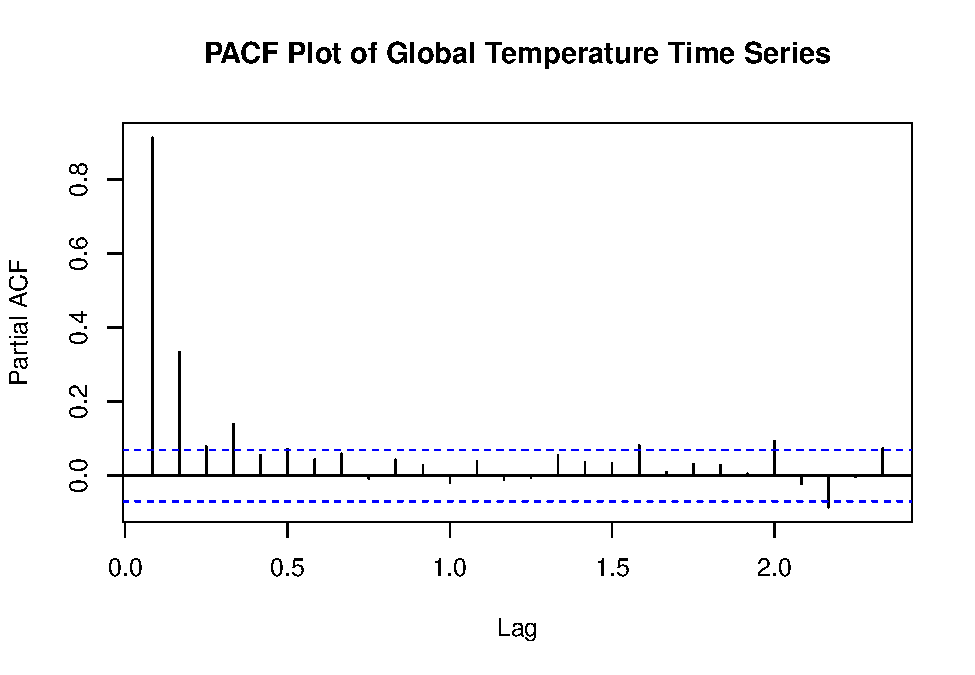
\includegraphics{431-Time-Series_files/figure-latex/unnamed-chunk-15-1.pdf}

What should we look for in this plot? The primary goal is to look for the number of significant spikes outside of the blue confidence intervals. In this plot, I would determine there to be 2 spikes, one at 0.1 and the other at 0.3. The spike at the 0 does not count and any spikes outside of the blue later in the plot are likely due to random error. Therefore, this looks like an AR(2) model.

Let's look at an AR(2) model for the global temp time series. You can use the \emph{ar()} function in R; however, I recommend using the \emph{Arima()} function from the \textbf{forecast} package because we'll be using it later on in this chapter.

\begin{Shaded}
\begin{Highlighting}[]
\CommentTok{# the first index in the order argument represents the order of the AR(2) model}
\NormalTok{ar.model <-}\StringTok{ }\KeywordTok{Arima}\NormalTok{(temp.ts, }\DataTypeTok{order =} \KeywordTok{c}\NormalTok{(}\DecValTok{2}\NormalTok{,}\DecValTok{0}\NormalTok{,}\DecValTok{0}\NormalTok{))}
\NormalTok{ar.model}
\end{Highlighting}
\end{Shaded}

\begin{verbatim}
## Series: temp.ts 
## ARIMA(2,0,0) with non-zero mean 
## 
## Coefficients:
##         ar1     ar2    mean
##       0.588  0.3700  0.2697
## s.e.  0.033  0.0332  0.0908
## 
## sigma^2 estimated as 0.01234:  log likelihood=617.65
## AIC=-1227.3   AICc=-1227.25   BIC=-1208.6
\end{verbatim}

So, this is our AR(2) model. How do we know it it's a good model? We will compute other models first and then talk about how to compare them.

\textbf{Moving Average Model: MA(q)}

The moving average model is a time series model that accounts for very short-run autocorrelation. It basically states that the next observation is the mean of every past observation. The order of the moving average model, q, can usually be estimated by looking at the ACF plot of the time series. Let's take a look at the ACF plot again.

\begin{Shaded}
\begin{Highlighting}[]
\NormalTok{acf.plot <-}\StringTok{ }\KeywordTok{acf}\NormalTok{(temp.ts, }\DataTypeTok{lag.max =} \DecValTok{300}\NormalTok{)}
\end{Highlighting}
\end{Shaded}

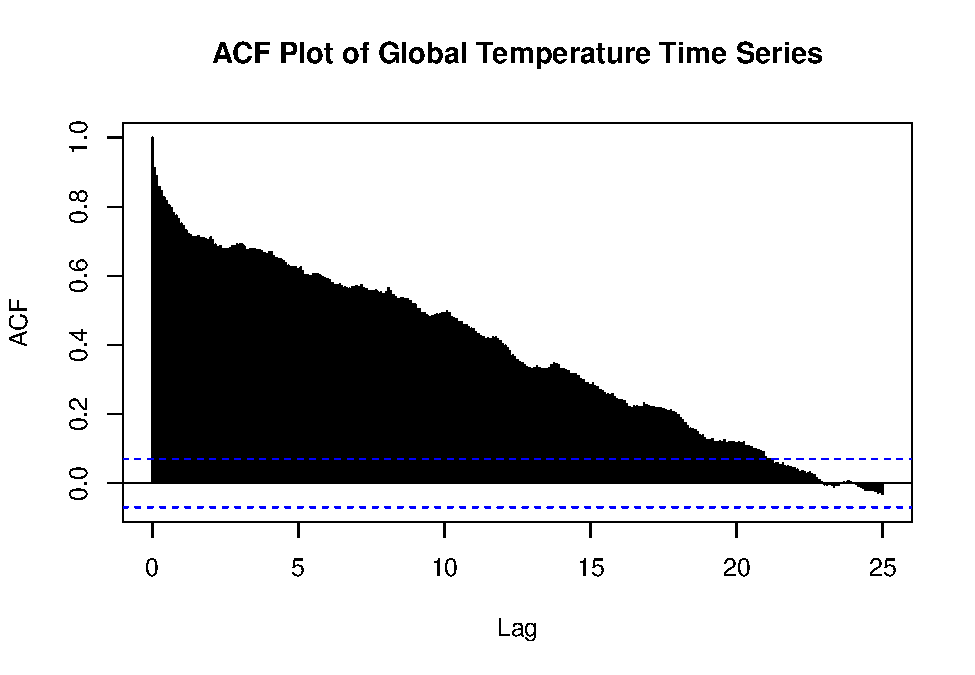
\includegraphics{431-Time-Series_files/figure-latex/unnamed-chunk-18-1.pdf}

As we have seen, this ACF plot takes a very long time to converge. What does this mean? This likely means that making a moving average model of this time series would not fix the problem of not having a stationary time series. Thus, the MA model will likely not be a good model to forecast with; however, for the sake of comparing models, we will still view one.

Let's looks at an MA(5) model. Usually, we would pick order, q, for how many signficiant spikes there are in the ACF plot; however, considering that there are hundreds in this example, we will just use 5. \textbf{Careful:} if you use too high of an order, it can result in too many predictors in the model which may cause overfitting.

\begin{Shaded}
\begin{Highlighting}[]
\CommentTok{# the third index in the order argument represents the order of the MA(5) model.}
\NormalTok{ma.model <-}\StringTok{ }\KeywordTok{Arima}\NormalTok{(temp.ts, }\DataTypeTok{order =} \KeywordTok{c}\NormalTok{(}\DecValTok{0}\NormalTok{,}\DecValTok{0}\NormalTok{,}\DecValTok{5}\NormalTok{))}
\NormalTok{ma.model}
\end{Highlighting}
\end{Shaded}

\begin{verbatim}
## Series: temp.ts 
## ARIMA(0,0,5) with non-zero mean 
## 
## Coefficients:
##          ma1     ma2     ma3     ma4     ma5    mean
##       0.8056  0.8663  0.6675  0.5288  0.2949  0.2479
## s.e.  0.0349  0.0420  0.0402  0.0340  0.0299  0.0197
## 
## sigma^2 estimated as 0.01799:  log likelihood=470.17
## AIC=-926.35   AICc=-926.2   BIC=-893.61
\end{verbatim}

We didn't cover the actual formulas and notation of the models; however, if this interests you, view this webiste below for more details.
\href{https://maryclare.github.io/atsa/content/notes/notes_3.pdf}{\textbf{Formulas Behind AR and MA Models}}

The orders of the AR and the MA models or usually picked by the number of significant spikes in the PACF and ACF plots respectively; however there are other conditions as well that can be seen if you click \href{https://people.duke.edu/~rnau/arimrule.htm}{\textbf{here}}.

\hypertarget{arma-arima-and-sarima}{%
\section{ARMA, ARIMA, AND SARIMA}\label{arma-arima-and-sarima}}

The autoregressive moving average model (ARMA), autoregressive integrated moving average model (ARIMA) and the seasonal autoregressive integrated moving average model (SARIMA) are also commonly used models in time series analysis. Evidently, they all come from the same family. Thus, we will explain the small differences between them.

\textbf{Autoregressive Moving Average Model: ARMA(p,q)}

Autoregressive moving average models are simply a combination of an AR model and an MA model. Let's take a look at what our ARMA model would be.

We are going to build an ARMA(2,5) model by simply using the two orders from the previous models.

\begin{Shaded}
\begin{Highlighting}[]
\NormalTok{arma.model <-}\StringTok{ }\KeywordTok{Arima}\NormalTok{(temp.ts, }\DataTypeTok{order =} \KeywordTok{c}\NormalTok{(}\DecValTok{2}\NormalTok{,}\DecValTok{0}\NormalTok{,}\DecValTok{5}\NormalTok{))}
\NormalTok{arma.model}
\end{Highlighting}
\end{Shaded}

\begin{verbatim}
## Series: temp.ts 
## ARIMA(2,0,5) with non-zero mean 
## 
## Coefficients:
##          ar1      ar2      ma1     ma2      ma3     ma4      ma5    mean
##       1.8305  -0.8306  -1.3337  0.4087  -0.1512  0.1674  -0.0684  0.4220
## s.e.  0.0635   0.0634   0.0720  0.0663   0.0602  0.0591   0.0381  0.4206
## 
## sigma^2 estimated as 0.01158:  log likelihood=644.73
## AIC=-1271.45   AICc=-1271.22   BIC=-1229.37
\end{verbatim}

\textbf{Autoregressive Integrated Moving Average Model: ARIMA(p,d,q)}

This model is the same as the previous, except now it has this weird d argument. What does this d stand for? d represents the number of nonseasonal differences needed for stationarity. Simply, d just makes nonstationary data stationary by removing trends!

How do you pick your differencing term?

Usually, small terms are picked for the differencing term. If you pick too high, you will likely cause your model to incorrectly represent your data. Some general rules for picking your differencing term are that differencing should not increase your variance and the autocorrelation of the model should be less than -0.5.

Thus, I tried a few differencing terms and concluded that \(d=1\) would be best for the model as it had the lowest variance and the autocorrelation was less than -0.5.

\begin{Shaded}
\begin{Highlighting}[]
\NormalTok{arima.model <-}\StringTok{ }\KeywordTok{Arima}\NormalTok{(temp.ts, }\KeywordTok{c}\NormalTok{(}\DecValTok{2}\NormalTok{, }\DecValTok{1}\NormalTok{, }\DecValTok{5}\NormalTok{))}
\NormalTok{arima.model}
\end{Highlighting}
\end{Shaded}

\begin{verbatim}
## Series: temp.ts 
## ARIMA(2,1,5) 
## 
## Coefficients:
##          ar1     ar2      ma1      ma2     ma3     ma4     ma5
##       0.1022  0.6468  -0.6046  -0.6056  0.1762  0.0520  0.0157
## s.e.  0.2056  0.1859   0.2096   0.2859  0.1040  0.0581  0.0517
## 
## sigma^2 estimated as 0.01156:  log likelihood=645.66
## AIC=-1275.33   AICc=-1275.14   BIC=-1237.93
\end{verbatim}

\textbf{Seasonal Autoregressive Integrated Moving Average Model: SARIMA(p,d,q)(P,D,Q)s}

The SARIMA model is an extension of the ARIMA model. The only difference now is that this model added on a seasonal component. As we saw, ARIMA is good for making a non-stationary time series stationary by adjusting the trend. However, the SARIMA model can adjust a non-stationary time series by removing trend and seasonality.

As we know:

\begin{itemize}
\tightlist
\item
  p - the order of the autoregressive trend
\item
  d - the order of the trend differencing
\item
  q - the order of the moving average trend
\end{itemize}

What do (P,D,Q)s mean?

\begin{itemize}
\tightlist
\item
  P - the order of the autoregressive seasonality
\item
  D - the order of the seasonal differncing
\item
  Q - the order of the moving average seasonality
\item
  s - the number of periods in your season
\end{itemize}

How do you pick these new terms?

There are several ways to pick these orders; however, when trying to use the SARIMA model in practice, it is likely best to let R or other software estimate the parameters for you. This article attached \href{https://medium.com/@rrfd/sarima-modelling-for-car-sharing-basic-data-pipelines-applications-with-python-pt-1-75de4677c0cd\#:~:text=SARIMA\%20models\%20are\%20a\%20general,a\%20constant\%20mean\%20and\%20variance.}{\textbf{here}} mentions this in more detail.

In our example, we may not have a SARIMA model because our time series did not have seasonality. Therefore, it may follow a SARIMA(2,1,5)(0,0,0)12.

The s term would be 12 because there would be 12 periods (months) in the season if we had seasonality. We will still follow through with an example. We can use the sarima function from the \textbf{astsa} package in R.

\begin{Shaded}
\begin{Highlighting}[]
\NormalTok{sarima.model <-}\StringTok{ }\KeywordTok{sarima}\NormalTok{(temp.ts, }\DecValTok{2}\NormalTok{,}\DecValTok{1}\NormalTok{,}\DecValTok{5}\NormalTok{,}\DecValTok{0}\NormalTok{,}\DecValTok{0}\NormalTok{,}\DecValTok{0}\NormalTok{,}\DecValTok{12}\NormalTok{)}
\end{Highlighting}
\end{Shaded}

\begin{verbatim}
## 
## Call:
## stats::arima(x = xdata, order = c(p, d, q), seasonal = list(order = c(P, D, 
##     Q), period = S), xreg = constant, transform.pars = trans, fixed = fixed, 
##     optim.control = list(trace = trc, REPORT = 1, reltol = tol))
## 
## Coefficients:
##          ar1     ar2      ma1      ma2     ma3     ma4    ma5  constant
##       0.1286  0.6396  -0.6452  -0.5892  0.1750  0.0575  0.014    0.0012
## s.e.  0.2465  0.2227   0.2505   0.3498  0.1224  0.0628  0.055    0.0002
## 
## sigma^2 estimated as 0.0113:  log likelihood = 650.7,  aic = -1283.4
\end{verbatim}

Now that we have 5 different models, which one do you choose?

Often, this can be done simply by looking at the Akaike Information Criterion (AIC) or Bayesian Information Criterion (BIC). In our example, we will be looking at the AIC. Generally, a smaller AIC means the model fits the time series better.

If you check the output for each model, you will see they all have an AIC value. I will reprint them below as well.

\begin{verbatim}
##                    Model      AIC
## 1                  AR(2) -1227.30
## 2                  MA(5)  -926.35
## 3              ARMA(2,5) -1271.45
## 4           ARIMA(2,1,5) -1275.33
## 5 SARIMA(2,1,5)(0,0,0)12 -1283.40
\end{verbatim}

As we can see, the SARIMA model actually had the lowest AIC, thus we would conclude that the SARIMA made the time series stationary and is most sutiable for forecasting. However, as I mentioned before; when it comes to finding the best model, R or other software is likely the best. Thus, we will use the \emph{auto.arima()} function from the \textbf{forecast} package that will automatically select orders for us! In practice, I definitely recommend using this rather than going through each model and testing different orders.

\begin{Shaded}
\begin{Highlighting}[]
\NormalTok{best.model <-}\StringTok{ }\KeywordTok{auto.arima}\NormalTok{(temp.ts)}
\NormalTok{best.model}
\end{Highlighting}
\end{Shaded}

\begin{verbatim}
## Series: temp.ts 
## ARIMA(2,1,3)(1,0,0)[12] with drift 
## 
## Coefficients:
##           ar1     ar2      ma1      ma2     ma3     sar1   drift
##       -0.0069  0.6955  -0.5143  -0.6984  0.2307  -0.0304  0.0012
## s.e.   0.1027  0.0954   0.1128   0.1549  0.0759   0.0371  0.0002
## 
## sigma^2 estimated as 0.01142:  log likelihood=650.08
## AIC=-1284.15   AICc=-1283.97   BIC=-1246.76
\end{verbatim}

As we can see, this model that was selected for us, SARIMA(2,1,3)(1,0,0)12, has the lowest AIC at -1284.15. We will continue to use this model in the next chapter as we dive into forecasting.

\hypertarget{forecasting}{%
\chapter{Forecasting}\label{forecasting}}

Now that we covered the fundamentals of time series analysis, we finally get to immerse ourselves in forecasting!

\hypertarget{what-is-forecasting}{%
\section{What is Forecasting?}\label{what-is-forecasting}}

Forecasting is simply the process of using past data values to make educated predictions on future data values. As stated in the last chapter, the time series should be stationary if you want to make well-informed predicitons. This can be done by fitting an arima model by using the \emph{auto.plot()} function in the \textbf{forecast} package. Then, all you have to do is apply the \emph{forecast()} function to get your prediction! The \emph{forecast()} function can take in another argument along with your model. You can also input h, the number of predicted time periods you want. This function is very practical for real world analysis of time series.

Forecasting is done in so many fields around the world. You will often see forecasting in the business and financial field for companies that want to predict their profit or expenses. Forecasting can be used to predict stock prices as well! You will see it in the environemntal field, such as this current example with global warming. The economic field also heavily uses time series and forecasting to predict how societies will behave. This is just a few examples of numerous time series and forecasting uses in the real world.

\hypertarget{example-global-temperature}{%
\section{Example: Global Temperature}\label{example-global-temperature}}

Let's forecast with our global temperature data now. As we saw, we fit the data with a SARIMA(2,1,3)(1,0,0)12. Now that we have our model, we can simply use the forecast(ts, h) function from the \textbf{forecast} package. As mentioned, h represents the number of observations we want to predict into the future. Let's say we want to predict 5 years into the future. Since our data ended in December 2016, the next 5 years will include each month from January 2017 to December 2022. Moreover, since our observations were every month, we can set h to \(12 * 5 = 60\). Let's see what happens.

\begin{Shaded}
\begin{Highlighting}[]
\NormalTok{forecast.data <-}\StringTok{ }\KeywordTok{forecast}\NormalTok{(best.model, }\DataTypeTok{h =} \DecValTok{60}\NormalTok{)}

\KeywordTok{autoplot}\NormalTok{(forecast.data, }\DataTypeTok{ts.colour =} \StringTok{"dodgerblue4"}\NormalTok{, }\DataTypeTok{predict.colour =} \StringTok{"red"}\NormalTok{) }\OperatorTok{+}
\StringTok{  }\KeywordTok{ggtitle}\NormalTok{(}\StringTok{"Forecasted Data for the next 60 months"}\NormalTok{) }\OperatorTok{+}\StringTok{ }
\StringTok{  }\KeywordTok{ylab}\NormalTok{(}\StringTok{"Average Temperature Difference (Celsius)"}\NormalTok{) }\OperatorTok{+}
\StringTok{  }\KeywordTok{theme_classic}\NormalTok{()}
\end{Highlighting}
\end{Shaded}

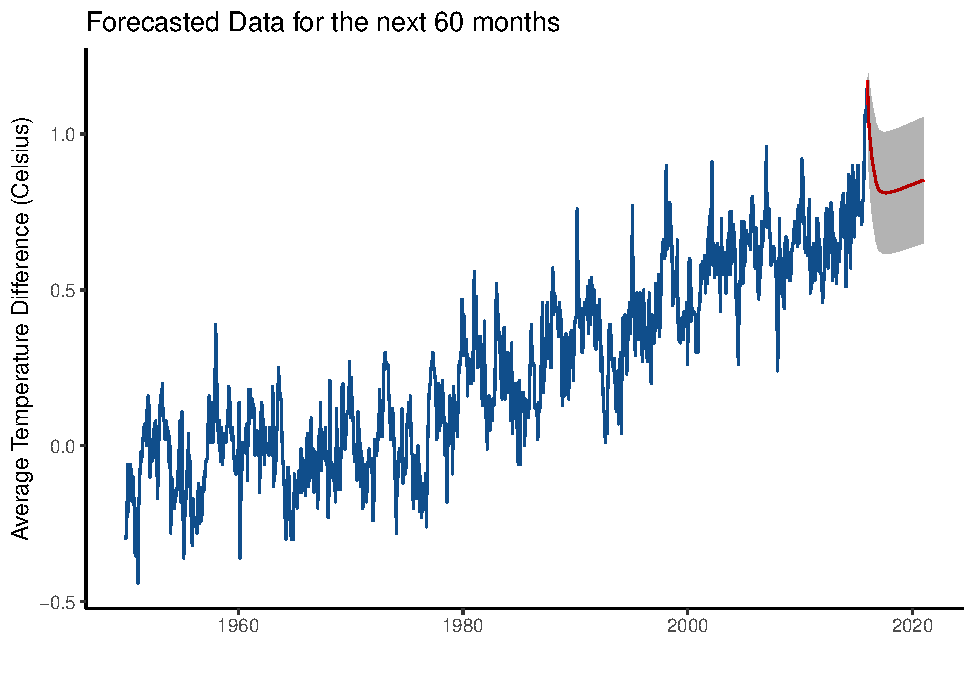
\includegraphics{431-Time-Series_files/figure-latex/unnamed-chunk-28-1.pdf}

The original time series is depicted in dark blue and the predicted data is represented by the red line. The grey shading around the predicted values represents the 95\% confidence interval. This simply states that we are 95\% percent confident that the data point at time \emph{t} will fall between two bounds. You can change the confidence bands in the forecast function and even view the confidence interval bounds in the forecasted object.

What can you take away from this forecasted model?

It looks as it the average temperature difference will drop in 2017; however, it seems that it will gradually rise again. This is fairly consistent in what we see in the rest of the data. It seems in the past 66 years, the temperatue decreases every once in a while, but then gradually rises. This looks like it's a fairly good prediction.

There are many other methods to create a model for your time series data. You can also check which is the best predictor by looking at the mean absolute percentage error (MAPE). This is beyond the scope of this short tutorial, but I encourage you to learn more about it \href{https://www.pluralsight.com/guides/time-series-forecasting-using-r}{\textbf{here}}.

\hypertarget{summary}{%
\chapter{Summary}\label{summary}}

Throughout this book, we scraped the surface of time series analysis. In review, we covered:

\begin{itemize}
\tightlist
\item
  What is a time series?

  \begin{itemize}
  \tightlist
  \item
    A time series is a series of data points over time.
  \end{itemize}
\item
  Components of a time series

  \begin{itemize}
  \tightlist
  \item
    Trend, seasonality, random white noise.
  \end{itemize}
\item
  Stationarity

  \begin{itemize}
  \tightlist
  \item
    Defined as constant means and varaince throughout the series.
  \item
    Time series should be stationary when forecasting.
  \item
    Must fit a model to the time series to detrend and deseasonalize the series.
  \end{itemize}
\item
  AR and MA models

  \begin{itemize}
  \tightlist
  \item
    The autoregressive model uses observations from preivous time steps as input to a regression equations to predict the value at the next step.
  \item
    The moving average model is a time series model that accounts for very short-run autocorrelation.
  \item
    You should use the ACF and PACF plots to determine the order of these.
  \item
    These models only work on stationary data.
  \end{itemize}
\item
  ARMA, ARIMA, and SARIMA Models

  \begin{itemize}
  \tightlist
  \item
    ARMA models are a combination of AR and MA models and only works on stationary data.
  \item
    ARIMA models are the same as an ARMA model, but there is a differencing term to detrend the non-stationary data.
  \item
    SARIMA models are the same as an ARIMA model, but there are seasonal terms to detrend and deseasonalize the non-stationary data.
  \item
    \textbf{In practice, use the auto.arima() function from the forecast package.}
  \end{itemize}
\item
  Forecasting

  \begin{itemize}
  \tightlist
  \item
    Defined as using the previous data points to make a well-informed predictions of the future.
  \item
    The \textbf{forecast()} function is best to predict your time series.
  \end{itemize}
\end{itemize}

These is just a small chunk of what time series has to offer. There are many other components and different techniques to detrend and deseasonalize your time series that we didn't talk about in this book. I hope this short tutorial assisted you in learning the basics of time series and equipped you with the tools to forecast.

Now that you have learned the basics, make sure to check out our correspoding API package and Stock Shiny App to explore real world uses of time series You will be able to look at the series of real time stock prices for companies around the world!

\href{https://people.duke.edu/~rnau/arimrule.htm}{Duke University, \emph{Summary of Rules for Identifying ARIMA Models}}

\href{https://datahub.io/core/global-temp}{\emph{Global Temperature Time Series Data}}

\href{https://nwfsc-timeseries.github.io/atsa-labs/}{Holmes, Scheuerell, \& Ward, \emph{Applied Time Series Analysis}}

\href{https://otexts.com/fpp2/}{Hyndman \& Athanasopoulos, \emph{Forecasting Principles and Practice}}

\href{https://rpubs.com/riazakhan94/arima_with_example}{Khan, \emph{ARIMA Model for Forescating - Example in R}}

\href{https://towardsdatascience.com/the-complete-guide-to-time-series-analysis-and-forecasting-70d476bfe775}{Towards Data Science, \emph{The Complete Guide to Time Sereis Analysis and Forecasting}}

  \bibliography{book.bib,packages.bib}

\end{document}
